\begin{frame}
  \LectureNo{1}
  \maketitle
\end{frame}

\begin{frame}{Overview}
\tableofcontents[pausesections]
\end{frame}

\section{0. Course Admin}
\begin{frame}{0. Course Admin}

  \begin{itemize}[<+->]
	\item You got to do it.
  \end{itemize}

\end{frame}

\begin{frame}{Course Material}

	The course material consists of:

	\begin{itemize}[<+->]
	  \item the syllabus
	  \item the lecture notes
	  \item the slides
	  \item the textbook ``How to Think Like a Mathematician''
			\begin{center}
			  \url{http://www.kevinhouston.net/httlam.html}
			\end{center}
	  \item supplementary readings (optional, but recommended)
	\end{itemize}

	\emph{Watch out}: The course material will be updated throughout the semester. Go to GitHub fetch the latest version!

	\begin{center}
	  \url{https://github.com/jkorb/KI1V13001}
	\end{center}

\end{frame}
\begin{frame}{Exercises and Assignments}

``{\it The best way to learn logic is to do exercises. A lot of exercises.}''
\begin{flushright}
Any logic professor, ever.
\end{flushright}

	\begin{itemize}[<+->]

		\item Each lecture covers one chapter of the notes.

		\item Exercises are at the end of each chapter.

		\item Homework is marked $[h]$ and is due in the workgroups.

		\item Your TA gives \emph{formative feedback}.

		\item \textbf{You have to present once, otherwise you fail! (ND)}

		\item There's a syllabus quiz on BB (perfect score to pass, unlimited attempts)

		\item Know who your TA is.

	\end{itemize}

\end{frame}

\begin{frame}{Teaching Assistants}

You can find out which is your workgroup number via blackboard or \url{https://mytimetable.uu.nl}:
{\small \begin{center}
\TAS
\end{center}}


\end{frame}

\begin{frame}{Grading}

	\begin{itemize}[<+->]

		\item There are two exams: midterm (MT, digital) and end term (ET, analog).

		\item Dates:

					\begin{itemize}
						\item \Tussentoets
						\item \Eindtoets
					\end{itemize}

		\item Your grade will be calculated according to the following formula:

			\[Grade=\frac{1}{2}\times MT+\frac{1}{2}\times ET\]

		\item \begin{enumerate}[<+->]

				\item If $Grade\geq 5.5$, then pass. \emph{No improvements!}

				\item If $4.0\leq Grade<5.5$, then you may take the resit.

				\item If $Grade<4.0$, then fail. \emph{No resit!}

			\end{enumerate}

		\item Resit: \Herkansing

		\item If eligible, you can resit \emph{either} the midterm \emph{or} the end term.

	\end{itemize}

\end{frame}

\begin{frame}{Humboldtian Model of Higher Education}

		\begin{center}
			\begin{tabular}{c}
			 	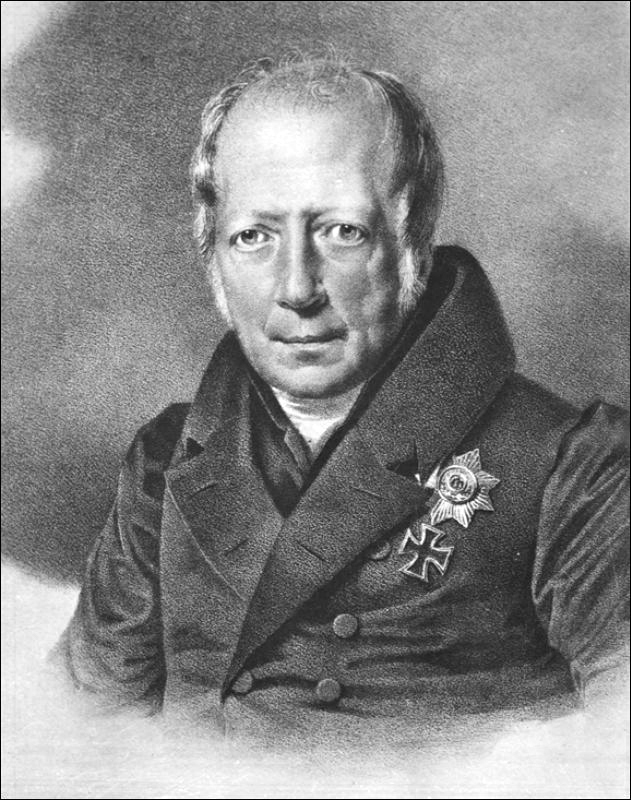
\includegraphics[height=12ex]{humboldt.jpg}\\
				Wilhelm von Humboldt\\
				{\tiny $\not\hspace{-1ex}\textcopyright$ Lithography by Franz Kr\"uger, work in public domain}
			\end{tabular}
		\end{center}

		\begin{quote}
			[At university], the teacher does not exist for the sake of the student; both teacher and student have their justification in the common pursuit of knowledge.
		\end{quote}

\end{frame}

\begin{frame}{Study Attitude ---  University $\neq$ High-school}

	\begin{center}
			\begin{tabular}{c}
			 	
\includegraphics[width=30ex]{non-scholae.jpg}\\
				{\tiny \textcopyright~by wikipedia user \texttt{Atamari}, CC BY-SA 3.0, image cropped}
			\end{tabular}
		\end{center}

	\begin{center}
		\begin{tabular}{ c | c }
		``High-school'' mindset & University mindset\\\hline
		Studying for exams & Studying for life\\
		Guided studying & Independent studying\\
		Passive & Active\\
		Memorization & Understanding\\

		\end{tabular}
	\end{center}

\end{frame}

\begin{frame}{Students and Teachers}

	\begin{itemize}[<+->]

		\item I, the teacher, am not here to simply \emph{tell} you things, I'm here to \emph{help} you understand them.

		\item You, the student, are an \emph{autonomous individual}:

			\begin{itemize}[<+->]

				\item you make use of your \emph{reason}
				\item you \emph{determine} your own goals
				\item you're \emph{responsible} for your own success
				\item \dots

			\end{itemize}

		\item You are a \emph{citizen of the (academic) world}:

			\begin{itemize}[<+->]

					\item you interact with other autonomous individuals, \emph{regardless of their social and cultural background}
					\item you treat others as \emph{equals}
					\item \dots
			\end{itemize}

	\end{itemize}

\end{frame}

\begin{frame}{Study Load}

	\begin{itemize}[<+->]

		\item This is a 7.5 ECTS course. One ECTS is worth 28 hours:
		\[7.5\times 28=210\]

		\item We have 68 contact hours + 6 hours of exam:
		\[210-68-6=136\]

		\item Preparing a lecture (reading notes) or workgroup (doing exercises) takes ca. 2 hours. There are 17 lectures and workgroup meetings:
		\[136-2\times 17-2\times 17=68\]

		\item This leaves \textbf{68 hours} for independent self-study:

			\begin{itemize}[<+->]

				\item re-read the material

				\item do extra exercises

				\item read extra material

				\item \dots

			\end{itemize}

	\end{itemize}

\end{frame}

\begin{frame}{Contact}

  By default, for any admin matters such as:
  \begin{itemize}[<+->]

	\item workgroup change
	\item sick notes
	\item extra time during exams
	\item  \dots
  \end{itemize}
  contact:
  \begin{itemize}
	\item \href{mailto:inleiding.logica@uu.nl}{\texttt{inleiding.logica@uu.nl}}
  \end{itemize}

  Please don't use our personal email addresses (it's for your own good)!

\end{frame}

\section{1. Introduction}
\begin{frame}{1. Introduction}

	\begin{center}
		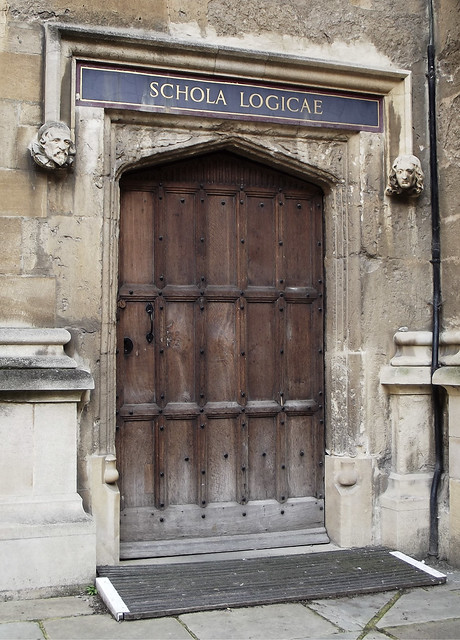
\includegraphics[width=25ex]{schola-logicae}\\
		{\tiny \textcopyright~James Clark, \url{https://www.flickr.com/photos/cathedralcityguide/14023988013}, CC BY-SA 2.0, no changes made}

	\end{center}

\end{frame}

\subsection{1.1 Valid Inferences}
\begin{frame}{1.1 Valid Inferences}

	\begin{itemize}[<+->]

		\item (1.1.1)  Logic is concerned with reasoning, more specifically \emph{valid} reasoning.

		\item Quiz:

		\begin{center}
		\fbox{
		\begin{minipage}{.9\linewidth}

		\vspace{2ex}

		Information:

		\vspace{-2ex}

			\begin{center}

				\begin{tabular}{c c}

				\begin{minipage}{.5\linewidth}

					\begin{enumerate}

						\item Charles sees Betty



						\item Betty sees Albert

					\end{enumerate}

					\end{minipage}



				&

				\begin{minipage}{.5\linewidth}

					\begin{enumerate}

						\setcounter{enumi}{2}

						\item Charles is married



						\item Albert is unmarried

					\end{enumerate}

				\end{minipage}
		\\[2ex]
		\end{tabular}


	\end{center}



Is a married person looking at an unmarried person?

	\begin{enumerate}

		\item[]
			\begin{enumerate}[A.]



				\item Yes


\item No


\item Can't Tell

\item[]

\end{enumerate}
\end{enumerate}

	\end{minipage}
	}
	\end{center}

	%\item In a valid inference, the truth of the premises \emph{necessitates} the truth of the conclusion.

	\end{itemize}

\end{frame}

\begin{frame}{Answer: A!}


Either \begingroup\color{structure}(a) \endgroup Betty is married or  \begingroup\color{structure}(b) \endgroup  Betty is unmarried.




\begin{enumerate}[(a)]

\item If Betty is married, then a married person, Betty, is looking at an unmarried person, Albert.



\item If Betty is unmarried, then a married person, Charles, is looking at an unmarried person, Betty.

\end{enumerate}




In either case, a married person is looking at an unmarried person.

\end{frame}

\begin{frame}{Validity --- The Standard Account}

	\begin{itemize}

		\item (1.1.5) An inference is said to be \emph{valid} iff (`if and only if') in every possible situation where the premises are true, the conclusion is true as well.

		\item (1.1.6) It follows that an inference is \emph{invalid} iff there exists a possible situation in which the premises are true and the conclusion is false.

		\item \emph{Examples}:

		\begin{enumerate}[(1)]

		\item The letter is either in the left drawer or in the right drawer, and it's not in the left drawer. So, the letter is in the right drawer.

		\item If the ball is scarlet, then it's red, and the ball is red. So, the ball is scarlet.

	\end{enumerate}

	\end{itemize}

\end{frame}

\begin{frame}{Logical Theory}


	\begin{itemize}[<+->]

		\item We develop a \emph{mathematical} account of validity:

			\begin{itemize}

				\item (1.1.2--3) \emph{Syntax} --- the study of symbols (formal languages)

				\item (1.1.5--8) \emph{Semantics} --- the study of meaning (models and truth)

				\item (1.1.9--10) \emph{Proof theory} --- the study of inference (proof systems)

			\end{itemize}

		\item (1.1.4) We're \emph{about} logic (`object language') \emph{using} mathematics (`meta-language').

		\item The relation between logic and reasoning is like the relation between science and the world:

	\end{itemize}

	\begin{center}
		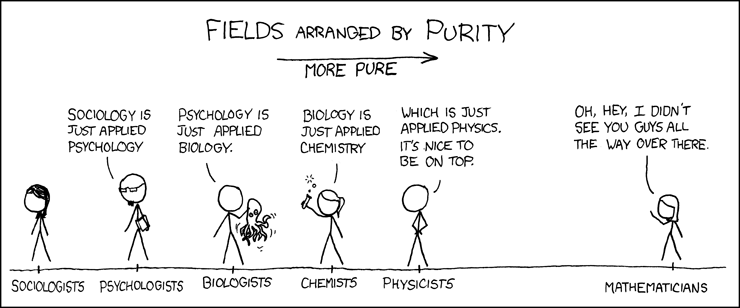
\includegraphics[width=30ex]{xkcd-purity}\\
		{\tiny \textcopyright~\url{https://www.xkcd.com/435/}, CC BY-NC 2.5}
		\end{center}

\end{frame}

\subsection{1.2 Propositional and First-Order Logic}
\begin{frame}{1.2 Propositional and First-Order Logic}

	\begin{itemize}


		\item (1.2.1--2) \emph{Propositional logic} deals with inferences using the sentential connectives: ``not,'' ``and,'' ``or,'' ``if \dots, then \dots,'' and so on.

		\item (1.2.3--4) First-order logic deals with all of the inferences inferences involving \emph{generality}:

			\begin{enumerate}[(1)]
		\setcounter{enumi}{2}

		\item This ball is scarlet and everything that's scarlet is red. So, this ball is red.

		\item The letter is in the left drawer. So there is something in the left drawer.

	\end{enumerate}

		\item To deal with generality, we need quantifiers: ``for all'' and ``there exists.''

		\item First-order logic subsumes propositional logic, but we'll deal with both.

	\end{itemize}

\end{frame}

\subsection{1.3 Classical Logic}
\begin{frame}{1.3 Classical Logic}

	\begin{itemize}

		\item (1.3.2) \emph{Consistency}: No statement is both true and false.

				\begin{center}
					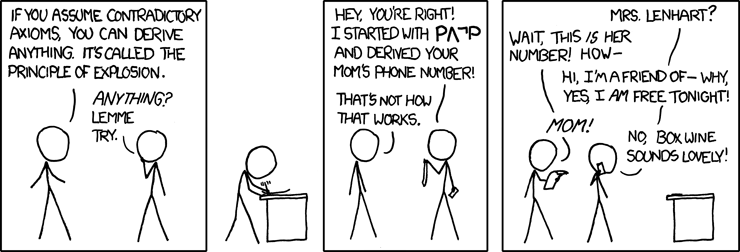
\includegraphics[width=30ex]{xkcd-explosion}\\[-1.8ex]
					{\tiny \textcopyright~\url{https://xkcd.com/704/}, CC BY-NC 2.5}
		\end{center}

		\item (1.3.5) \emph{Completeness}: Every statement is either true or false.

				\begin{center}
					
\includegraphics[width=30ex]{xkcd-tautology}\\[-1.8ex]
					{\tiny \textcopyright~\url{https://www.xkcd.com/703/}, CC BY-NC 2.5}
		\end{center}

		\item (1.3.6) A \emph{logical truth} is true in every situation. A \emph{logical falsehood} is false in every situation.

			\begin{itemize}

					\item Betty is either married or unmarried (logical truth).

					\item Betty is both married and unmarried (logical falsehood).

			\end{itemize}

	\end{itemize}

\end{frame}

\begin{frame}{Characteristics of Classical Logic}

	\begin{itemize}

		\item (1.3.8) Bivalence:

				\begin{description}

					\item[Bivalence.] For every model of a formal language, every statement of the language is either true or false in the model and never both.

				\end{description}


		\item (1.3.9) Some other characteristics:

			\begin{itemize}

				\item Only propositional and first-order logic, no necessity, likely truth, probability, \dots

				\item Standard account of validity as truth-preservation

				\item Taking ``if \dots, then \dots'' to be the \emph{material conditional}.

	\end{itemize}


		\item Non-classical logics deny some of these:

			\begin{itemize}

				\item (1.3.4) In \emph{paraconsistent} logic, we deny consistency.

				\item (1.3.7) In \emph{paracomplete} logic, we deny completeness.

				\item In \emph{modal logic}, we cover necessity and possibility.

				\item In \emph{non-monotonic logic}, we cover defeasible inference.

				\item \dots

			\end{itemize}

	\end{itemize}

\end{frame}

\subsection{1.4 Decidability}
\begin{frame}{1.4 Decidability}

	\begin{itemize}

		\item Hey, can't we automatize all this???

		\begin{center}
					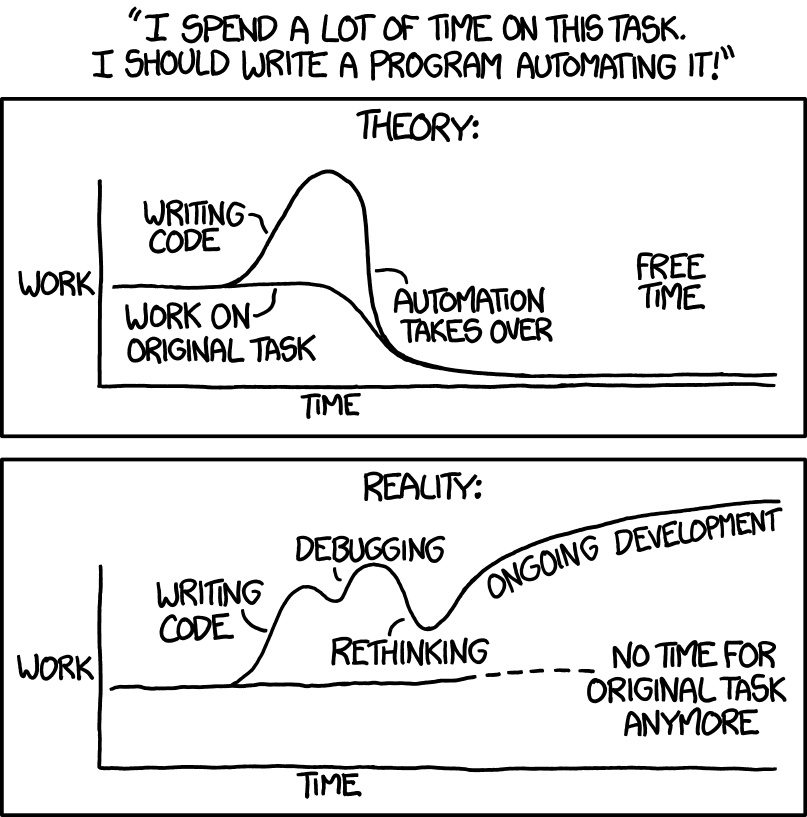
\includegraphics[width=25ex]{xkcd-automation}\\[-1.8ex]
					{\tiny \textcopyright~\url{https://www.xkcd.com/1319/}, CC BY-NC 2.5}
		\end{center}

		\item (1.4.2) Unfortunately, not!

			\begin{theorem}[Church-Turing] There is no effective algorithm that decides \emph{whether} a given inference in first-order logic is valid.

			\end{theorem}

	\end{itemize}

\end{frame}

\begin{frame}{Core Ideas (Lecture Version)}

\begin{itemize}

		\item You're not a high-school student anymore: you're an autonomous individual, a citizen of the world.

		\item An inference is valid iff in every situation in which the premises are true, so is the conclusion.

		\item Logical theory has three sub-disciplines: syntax, semantics, and proof theory.

		\item Propositional logic deals with the sentential connectives; first-order logic also with the quantifiers.

		\item In classical logic, we assume that every statement is either true or false and never both.

		\item Some logics are not decidable (e.g. first-order logic).

	\end{itemize}


\end{frame}

\begin{frame}

	\begin{center}
	{\huge\bf Thanks!}
	\end{center}

\end{frame}
